% Created 2017-02-09 jeu. 02:21
% Intended LaTeX compiler: pdflatex
\documentclass{article}
\usepackage{natbib}
\usepackage[french]{babel}
\usepackage[utf8]{inputenc}
\usepackage[T1]{fontenc}
\usepackage{graphicx}
\usepackage{longtable}
\usepackage{hyperref}
\usepackage{natbib}
\usepackage{amsmath,amssymb,amsthm,amsopn}
\usepackage{mathrsfs}
\usepackage{geometry}
\geometry{a4paper,left=2.5cm,top=2cm,right=2.5cm,bottom=2cm,marginparsep=7pt, marginparwidth=.6in}

\author{Li Honglin \\Maxime Buron}
\date{\today}
\title{Deep Structured Output Learning For Unconstrained Text Recognition}
\hypersetup{
 pdfauthor={Li Honglin Maxime Buron},
 pdftitle={Deep Structured Output Learning Dor Unconstrained Text Recognition},
 pdfkeywords={},
 pdfsubject={},
 pdfcreator={Emacs 24.5.1 (Org mode 9.0)}, 
 pdflang={French}}
\begin{document}

\maketitle
\tableofcontents
\section{Résumé du papier}
Nous avons choisi de travailler sur le papier intitulé Deep Structured Output Learning Dor Unconstrained Text Recognition de Max Jaderberg, Karen Simonnyan, Andrea Vedaldi et Andrew Zisserman. Voici un résumé de ce que nous en avons compris. L'article présente trois méthodes pour résoudre le problème suivant, dont la dernière combine les deux premières.
\subsection{introduction du problème}
Ce papier s'attaque au problème très général suivant : détecter et reconnaître du texte sur une image. Plus précisément, ce papier suppose la phase de détection est déjà réalisée, en d'autres termes l'on ne considère que des images contenant uniquement un seul mot sans autre contenu. Le sujet principal est donc la reconnaissance de mot, et particulièrement de mot sans contrainte, c'est à dire des mots qui ne sont pas obligatoirement issue d'une liste de vocabulaires.

\subsection{encodage de l'entrée}
Comme dit précedemment, l'entrée du problème est un image, seulement pour des questions de standardisation, notre algorithme nécessite des images de taille fixe $32\times100$ en noir et blanc. Malheuresement les images des ensembles de données ne sont pas toutes la même taille, c'est pourquoi elle sont étirées pour atteindre ces dimensions et cela sans préserver les proportions. Les images, une fois chargée sous forme de matrices de dimension $32 \times 100$ sont normalisées en leur soustrayant leur moyenne et en les divisant par leur écart type. 

\subsection{l'approche par caractère}
L'approche par caractère considère que chaque caractère identifié selon sa position indépendemment des autres caractères. 

La modélisation de la sortie de l'algorithme est une liste de $N_{max}$ distribution de probabilités,où $N_{max}$ est la longueur maximale qu'un mot sur une image en entrée. Les distribution de probalités modèlisent les lois de variables aléatoires à valeurs dans l'alphabet $C$ considèré pour identifier les mots augmenté par un caractère vide $\phi$. Un mot $\omega$ composé des caractères $c_1c_2\dots c_n$ avec $n\leq N_{max}$ est encodé par la suite de $N_{max}$ caractères suivantes $c_1, c_2, \dots,c_n,\phi,\dots,\phi$. La prédiction de l'algorithme pour une image donnée $x$ est alors l'encodage $\omega^*$ défini par :
$$ \omega^* = \text{arg} \max_{\omega} P(w|x) = \text{arg} \max_{c_1, c_2, \dots,c_{N_{max}}} \prod_{i=1}^{N_{max}} P(c_i|\Phi(x))$$
où $\Phi(x)$ est un ensemble de paramètres.

L'algorithme du calcul des distributions est constitué d'un réseau de neurore conditionnel, qui sera réutiliser dans la méthode suivante. Ce réseau de neurone est constitué de 5 couches convolutionnelles et 2 couches complétementement connectées de la dimension de l'image en entrée.

Au bout du réseau de neurones spécialisé pour cette méthode, il y a $N_{max}$ couches complétements connectées et indépendantes avec $|C|+1$ neurones où $C$ est l'alphabet de sortie. On peut alors interpréter les valeurs de chacune de ces couches comme les distributions de probabilités mentionnées plus haut.

En ce qui concerne la fonction de score $S_1$ de cette approche, on peut la définir de la manière suivante :
$$ S_1(\omega,x) = \log P(\omega|x)  = \sum_{i=1}^{N_{max}} S^i(c,x)$$
où $S^i$ est le logarithme de la probabilité que $i^e$ caractères de la sur l'entrée $x$ soit $c$ d'après l'algorithme.

Le réseau de neurones est entraîné par une descente de gradient stochastique.

\subsection{l'approche par sac de mots}

L'approche par sac de mots utilise la même entrée, que l'approche précédentes.

La sortie de cette approche est la probalité pour une sous-chaîne de caractères d'être présente dans l'image en entrée. On considère en particulier uniquement les sous-chaînes de taille inférieur à $N$ un entier, en pratique on a choisi 4. On définit le sac de mots d'un mot comme étant l'ensemble des sous-chaîne de caractères d'un mot. Pour des raisons pratiques, on ne considère que les sous-chaînes les plus présentes dans les datasets considérés et l'on nomme leur ensemble $G_N$.

L'algorithme pour déterminer cette probabilité utilise le même premier réseau de neurones de l'approche précédent, mais se terminer avec une unique couche complétement connectée possédant exactement un neurone pour chaque sous-chaîne de caractères de $G_N$. 

Ici la fonction de score $S_2$ peut être définie de la manière suivante :
$$S_2(\omega,x) = \sum_{i=1}^{|\omega|} \sum_{k=1}^{\min(N,|\omega| -i +1)} S_e(c_ic_{i+1}\dots c_{i+k-1},x)$$
où $\omega$ composé des caractères $c_1c_2\dots c_n$ et $S_e(c_ic_{i+1}\dots c_{i+k-1},x)$ est le logarithme de la probabilité d'avoir la sous-chaîne $c_ic_{i+1}\dots c_{i+k-1}$ dans l'entrée $x$. Si $s \notin G_N$, alors $S_e(s,x) = 0$

\subsection{l'approche jointe}
La méthode jointe effectue en parallèle est deux méthodes précédentes et définit un nouveau score $S$ pour une entrée $x$ définie par :
$$ S(\omega,x) = S_1(\omega,x) + S_2(\omega,x)$$

Encore une fois, une sortie pour cette approche est un mot qui maximise la fonction de score sachant l'entré $x$.

Ici, nous allons parler de la fonction du perte appliquée dans l'approche jointe, elle s'adapte facilement aux autres approches en remplaçant simplement $S$ par $S_1$ ou $S_2$. La function de perte utilisée ici est une fonction de perte de type Hinge. C'est à dire que la fonction de perte $L$ sur une entrée $x$ pour un mot $\omega$ est définie par :
$$ L(x,\omega) = \max_{\omega \neq \omega' } \max(0,\mu+ S(\omega',x) - S(\omega,x))$$
où $\mu$ est une marge fixée.

\subsection{les différents ensembles de données}

Les ensembles de données utilisés pour effectuer l'évaluation des différents approches sont les suivants
\begin{itemize}
\item ICDAR 2003
\item ICDAR 2013
\item Street View Text : textes extraits de Google Street View
\item Synth90k : textes générés par ordinateur
\end{itemize}

Le derniers ensemble de données est particulièrement important. Il sert d'ensemble d'entraînement, puisqu'il est assez important.

\section{La méthode choisie}

\subsection{Notre projet}
Nous avons choisi de réaliser la première approche, qui évalue les caractères les uns après les autres. Et nous avons décidé d'utiliser le dataset ICDAR2013, qui semble d'une taille et d'une difficulté convenable.

\begin{figure}[h]
  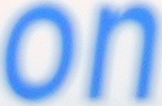
\includegraphics[scale=0.5]{./word_56.png}
  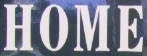
\includegraphics[scale=0.5]{./word_83.png}
  \caption{Exemple d'images en entrée}
\end{figure}

On remarque tout de suite la différence de taille des images, c'est pourquoi comme décrit précédemment les images sont déformées vers une taille précise et sauver dans une matrice à valeurs réelles. 

\section{L'implémentation}
Nous avons décidé d'utiliser Tensor Flow pour réaliser le réseau de neurones. 
\section{Les résultats}

\section{Conclusion}

\end{document}
